\documentclass[11pt, oneside]{article}   	% use "amsart" instead of "article" for AMSLaTeX format
\usepackage{geometry}                		% See geometry.pdf to learn the layout options. There are lots.
\geometry{letterpaper}                   		% ... or a4paper or a5paper or ... 
%\geometry{landscape}                		% Activate for for rotated page geometry
%\usepackage[parfill]{parskip}    		% Activate to begin paragraphs with an empty line rather than an indent
\usepackage{graphicx}				% Use pdf, png, jpg, or eps§ with pdflatex; use eps in DVI mode
								% TeX will automatically convert eps --> pdf in pdflatex		\documentclass[11pt, oneside]{article}   	% use "amsart" instead of "article" for AMSLaTeX format
	
\usepackage{amssymb}

\usepackage{listings}

\lstdefinelanguage
   [x64]{Assembler}     % add a "x64" dialect of Assembler
   [x86masm]{Assembler} % based on the "x86masm" dialect
   % with these extra keywords:
   {morekeywords={CDQE,CQO,CMPSQ,CMPXCHG16B,JRCXZ,LODSQ,MOVSXD, %
                  POPFQ,PUSHFQ,SCASQ,STOSQ,IRETQ,RDTSCP,SWAPGS, %
                  rax,rdx,rcx,rbx,rsi,rdi,rsp,rbp, %
                  r8,r8d,r8w,r8b,r9,r9d,r9w,r9b}} % etc.

\lstset{language=[x64]Assembler}

\begin{document}
\begin{titlepage}

\newcommand{\HRule}{\rule{\linewidth}{0.5mm}} % Defines a new command for the horizontal lines, change thickness here

\center % Center everything on the page
 
%----------------------------------------------------------------------------------------
%	HEADING SECTIONS
%----------------------------------------------------------------------------------------

\textsc{\LARGE Vrije Universiteit Brussel}\\[1.5cm] % Name of your university/college
\textsc{\Large Programming assignment}\\[0.5cm] % Major heading such as course name
\textsc{\large A game in assembly}\\[0.5cm] % Minor heading such as course title

%----------------------------------------------------------------------------------------
%	TITLE SECTION
%----------------------------------------------------------------------------------------

\HRule \\[0.4cm]
{ \huge \bfseries Othello}\\[0.4cm] % Title of your document
\HRule \\[1.5cm]
 
%----------------------------------------------------------------------------------------
%	AUTHOR SECTION
%----------------------------------------------------------------------------------------

\begin{minipage}{0.4\textwidth}
\begin{flushleft} \large
\emph{Authors:}\\
Kriz \textsc{De Logi} \\
Linda \textsc{de Corte} % Your name
\end{flushleft}
\end{minipage}
~
\begin{minipage}{0.4\textwidth}
\begin{flushright} \large

\end{flushright}
\end{minipage}\\[4cm]

%----------------------------------------------------------------------------------------
%	DATE SECTION
%----------------------------------------------------------------------------------------

{\large \today}\\[3cm] % Date, change the \today to a set date if you want to be precise
\vfill % Fill the rest of the page with whitespace

\end{titlepage}

\tableofcontents

\newpage

\section{Inleiding}

\subsection{De opdracht}
De opdracht was duidelijk van het begin, maak een spel in of een image encoder/decoder in assembly. De keuze ging uiteindelijk naar het maken van het spel Othello, ook wel bekend als Reversi op de oude Nokia telefoons. Het concept van het spel is duidelijk: een bord met 64 vakjes dient voor het plaatsen van steentjes die voor beide spelers resp. wit en zwart zijn ingekleurd. Bij het zetten van een witte steen worden alle zwarte stenen tussen de witte stenen en de juist geplaatste witte steen omgezet naar witte stenen. Dit wordt het 'stelen' van stenen genoemd. Hetzelfde principe geldt voor de omgekeerde situatie. De speler die aan het einde van het spel de meeste stenen op het bord heeft liggen wint het spel.
\subsection{Gebruiksaanwijzing}
Othello word in principe altijd gespeeld op een bord van 8 bij 8. Er zijn twee kleuren stenen: wit en zwart. E�n speler gebruikt zwarte stenen, de andere witte stenen. In het begin van het spel liggen er vier stenen in het midden, twee zwarte en twee witte die diagonaal van elkaar liggen. Het spel begint altijd met zwart, en de spelers maken om de beurt een zet.\newline\newline
Als een speler aan de beurt is plaatst hij een steen op het bord. Hij mag de stenen op een van de lege plaatsen op het bord zetten indien deze grenst aan een witte steen (ook diagonaal) waarbij in dezelfde richting nog een zwarte steen aanwezig is. M.a.w. er moet een 'diefstal' van stenen kunnen gebeuren bij het leggen van een steel. In deze versie van Othello kan je de mogelijke zetten herkennen aan de hand van vakjes die lichtgroen zijn gekleurd, terwijl de andere vakjes een donkergroene kleur hebben.\\
Het spel eindigt wanneer geen zetten meer mogelijk zijn: indien het speelveld volledig gevuld is met stenen of indien er voor beide partijen geen zetten meer kunnen gebeuren met 'diefstal'. Het spel is dan gewonnen door de speler met de meeste stenen op het veld.\newline\newline
De tussenstand tijdens het spelen is zichtbaar aan de rechterkant van het speelbord. Tevens is er aangeduid welke kleur aan zet is a.d.h. van een pijl.
Het spel kan be�indigt worden door te klikken op de rode knop die zich rechtsboven bevindt.


\newpage
\section{Het ontwerp}
\subsection{Design model}
\begin{figure}[htbp] %  figure placement: here, top, bottom, or page
   \centering
   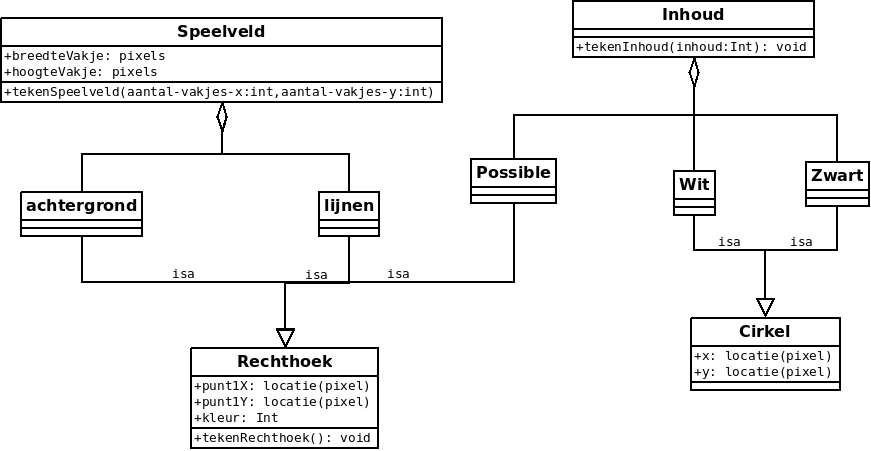
\includegraphics[width=7in]{graphicsdiagram.png} 
   \caption{Diagram van de graphics}
   \label{fig:example}
\end{figure}
~\newline
Zoals te zien is in het diagram, zijn alle tekeningen gebouwd op de rechthoek. Zodat elke tekening kan gemaakt worden zonder pixel per pixel te werken, maar dus a.d.v. combinaties van rechthoeken.
\newpage
\begin{figure}[htbp] %  figure placement: here, top, bottom, or page
   \centering
   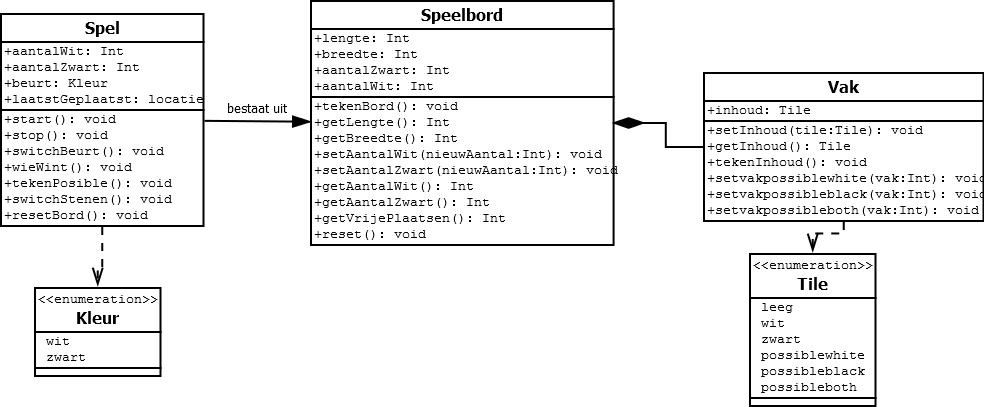
\includegraphics[width=7in]{othellodiagram.png} 
   \caption{Diagram van het spel}
   \label{fig:example}
\end{figure}
~\newline
Het spel bestaat uit een speelbord, die in dit project in een array van 64 bytes word voorgesteld, iedere byte bevat de informatie van de inhoud van het respectievelijke vak. Verder wordt er bijgehouden wie er aan de beurt is en hoeveel stenen ieder op het bord heeft liggen op dat moment. 

\newpage

\section{Problemen}
\subsection{Conditionele jumps}
Vrij snel na het schrijven van onze basis code kwamen we er achter dat een conditionele jump maar een beperkt bereik heeft. Wat vrij lastig is als er veel nodig zijn. Om dit te omzeilen hebben maken we gebruik van naamloze labels.\newline Voorbeeld:
\begin{lstlisting}
vergelijkzwart:
	mov ax, 0
	mov al, [speelveld+bx]
	cmp al, 2
	jne @F
	jmp swapstart
@@:
	cmp ax, 3
	jne @F
	jmp start
@@:
	jmp done
\end{lstlisting}

\subsection{Maximaal 3 tot 4 asm files}
Na het schrijven van alle code en het splitsen in verschillende files deed er zich een probleem voor. Namelijk dat CodeView niet kan werken met een argumentenlijst die langer is dan 255 tekens. Kortere namen gebruiken was ook geen optie, de code werd onleesbaar en lang. \newline
Na een gesprek met Tim Bruylants vernamen we dat we de functies beter konden samenvoegen in maximaal 3 a 4 files en dat variabelen maar een maal gedeclareerd mogen worden. Dit deden we vaker waardoor ons programma veel te veel geheugen nodig had.\\
  We hebben toen besloten om alle teken functies samen in een file te zetten, de logica functies in een file en een main file te maken. Zodanig dat alle functies mooi geclasseerd staan in een module.
 \newpage
\subsection{Elementen van de stack halen}
Het gebruiken van een array als manier voor het doorgeven van functiewaarden is niet optimaal. Hiervoor wordt het best gewerkt met de stack. De vooraf gepushte variabelen kunnen in een functie worden uitgelezen aan de hand van de base-pointer. Bij NEAR procedures moet er bij deze base-pointer 4 worden opgeteld, bij FAR procedures is dit 6. De laatst meegegeven waarde kan dan worden uitgelezen op locatie [0], de volgende op [2], enzovoort. (indien er bytes op de stack werden gepusht verhoogt dit getal uiteraard maar met 1, maar het gebruik van bytes op de stack word afgeraden).

\subsection{Elementen uit een array halen}
Het speelveld is een array van 64 bytes, de inhoud van een vakje uitlezen gebeurd a.d.h. van de mov ?l, [arraynaam+locatie] instructie.\newline
Voorbeeld:
\begin{lstlisting}
beurtblack:
	mov bx, VAK
	mov al, [speelveld+bx]			 
	cmp al, 4
		je vakjepossible		
		jmp bothcmp			
\end{lstlisting}

\subsection{Het plaatsen van elementen in array}
Het wegschrijven van een waarde in een array gebeurd analoog met het uitlezen. Namelijk a.d.h. van de instructie mov [arraynaam+locatie], ?l instructie.

\subsection{Compare problemen}
Compare is vaak een groot struikelblok geweest in het proces van het project.
\begin{lstlisting}
vergelijkvak:	
		mov bl, [beurt]
		cmp bl, 1
			je @F
			jmp vergelijkzwart		
\end{lstlisting}
In dit voorbeeld word een compare uitgevoerd op twee byte waarden, waarbij in sommige gevallen het programma niet meer loopte. Het gebruik van words in plaats van bytes bleek wel te werken:
\begin{lstlisting}
vergelijkvak:	
		mov bx, 0 
		mov bl, [beurt]
		cmp bx, 1
			je @F
			jmp vergelijkzwart
\end{lstlisting}

\subsection{Makkelijk fouten maken}
Assembly is een taal waar heel makkelijk een komma of een dubbelepunt word vergeten. Dus ipv:
	\begin{lstlisting}
	mov ax, 4			
\end{lstlisting}met komma na ax, schrijf je per ongeluk: \begin{lstlisting}
	mov ax 4			
\end{lstlisting}Dit lijkt een kleine fout, maar betekend wel dat heel het programma niet werkt en dit meteen terug geeft. Het oplossen is niet zo moeilijk want nmake geeft precies terug waar de fouten zitten. 

\subsection{Code View}
We hebben veel problemen gehad met de debugger die op Dosbox zit: Code View. In het begin kregen we niet alle functie calls te zien waardoor je nog niet wist wat er nu precies fout was. Na enige tijd kwamen we er achter dat je via F8 een oproep kan doen. Ook kwamen we er vrij laat pas achter dat je ook breakpoints kunt zetten, wat wel handig is als constant een functie aan het einde moet debuggen. Tot slot zijn we er achter gekomen dat Code View een heel duidelijk overzicht heeft van alle functies in assembler, wat ons tot een paar oplossingen heeft geleid. Misschien een goed idee om volgend jaar mee te geven aan de studenten.

\subsection{Overzichtelijkheid}
Omdat assembly zelf een hele on-overzichtelijke taal is waar je zonder uitleg niet veel van kunt maken was het samenwerken af en toe wel lastig. Daarom hebben we snel besloten om een paar regels op stellen voor overzichtelijkheid:
\begin{enumerate}
\item Voor de start van een procedure moet en vak waarin de naam staat, de uitleg en wat er eventueel in welke volgorde gepusht dient te worden.
\item Aan het eind van een procedure komt een lijn.
\item Bij een loop (na een label wordt er ingesprongen)
\subitem Voorgegaan met een lijntje met de naam van de loop.
\subitem Na de laatste jump, in dat deel van de code, sluit dit ook af met een korte lijn.
\item Na een compare wordt er ingesprongen op de volgende manieren:
\subitem Een conditionele jump fungeert als true tak en wordt ingesprongen. 
\subitem De insprong blijft tot de volgende jump of label, die als false tak fungeert, behalve indien 
\subitem er een nieuwe compare plaats vindt. 
\item Langs alle code, aan de rechterkant. Wordt er zo volledig mogelijk commentaar geplaatst op een verticale lijn.
\end{enumerate}


\newpage
\section{Slotwoord}



\end{document}  